\documentclass[11pt]{article}

% --- Packages ---
\usepackage[utf8]{inputenc}
\usepackage[T1]{fontenc}
\usepackage{amsmath,amssymb,amsthm}
\usepackage{algorithm}
\usepackage{algorithmic}
\usepackage{graphicx}
\usepackage{hyperref}
\usepackage{cleveref}
\usepackage{booktabs}
\usepackage{enumitem}
\usepackage[margin=1in]{geometry}
\usepackage{xcolor}
\usepackage{microtype}
\usepackage{float}
\usepackage{tikz}
\usetikzlibrary{arrows.meta,positioning,shapes.geometric,calc,fit,backgrounds}

% --- Theorem environments ---
\newtheorem{theorem}{Theorem}[section]
\newtheorem{lemma}[theorem]{Lemma}
\newtheorem{proposition}[theorem]{Proposition}
\newtheorem{corollary}[theorem]{Corollary}
\newtheorem{definition}[theorem]{Definition}
\newtheorem{axiom}{Axiom}[section]
\newtheorem{remark}[theorem]{Remark}

% --- Title ---
\title{SylannEngine v2: Affective Computation via Simplicial Resonance Fields\\with Hebbian Plasticity and Emergent Expression}

\author{
  Aylovelle S.S.\thanks{Correspondence: \texttt{aylovelle@icloud.com}}
}

\date{June 2026}

\begin{document}

\maketitle

% ============================================================
% ABSTRACT
% ============================================================
\begin{abstract}
We present SylannEngine v2, a computational framework for affective state evolution in AI companions based on simplicial resonance field dynamics. The architecture replaces sequential layer-by-layer pipelines with a fully-connected simplicial complex ($\Delta^6$ on 7 computation modules) where emotional state emerges through iterative resonance rather than feedforward computation. The system integrates six mechanisms from mathematical physics and neuroscience: (1)~Hebbian plasticity with homeostatic scaling for use-dependent channel strengthening; (2)~higher-order Kuramoto synchronization on simplicial complexes producing explosive phase transitions; (3)~Hopfield attractor landscapes encoding emotional memory as energy minima; (4)~harmonic identity extraction via Hodge theory preserving personality across perturbations; (5)~variational free energy minimization for precision-weighted belief updates; and (6)~expression as bifurcation---escaping an attractor basin when any single drive exceeds threshold. Two foundational principles govern the design: \emph{irreversibility} (scars accumulate, voids persist, history cannot be erased) and \emph{personality-driven computation} (all 441 coupling parameters derive deterministically from 7 personality dimensions). Experiments across 11 protocols with 10 repetitions each confirm: convergence within tier-specific iteration bounds, explosive synchronization under higher-order coupling, stable energy envelopes over 1500 ticks, and lossless tier hot-switching. The system operates at three performance tiers (lite: 42 channels/5ms, pro: 287 channels/40ms, max: 441 channels/50ms) with zero external dependencies at the lite tier.
\end{abstract}

% ============================================================
% 1. INTRODUCTION
% ============================================================
\section{Introduction}
\label{sec:intro}

The computational modeling of affective states in artificial agents faces a fundamental tension: systems must be rich enough to capture the temporal depth of emotional experience---where past wounds alter future processing and prolonged absence generates its own pressure---yet tractable enough for real-time deployment on commodity hardware. Existing approaches fall into two categories, each with critical limitations.

\paragraph{Classification-based systems.} The dominant paradigm in affective computing~\cite{picard1997} treats emotion as a classification problem over discrete labels (Ekman's basic emotions, Russell's circumplex). These systems are stateless: identical input produces identical output regardless of history. They cannot represent irreversibility, accumulated damage, or personality drift.

\paragraph{Neural network approaches.} Recurrent architectures (LSTMs, Transformers) can maintain state, but their internal representations are opaque, require training data, and provide no formal guarantees about bounded dynamics or personality preservation. The mapping from personality to behavior is implicit and uncontrollable.

We propose a third path: \emph{resonance field computation}, where emotional state emerges from the coupled dynamics of a simplicial complex rather than being computed by a feedforward pipeline or learned from data. The key insight is that a fully-connected topology with use-dependent plasticity naturally produces the properties required for relational AI:

\begin{enumerate}[leftmargin=*]
\item \textbf{Irreversibility.} Hebbian plasticity permanently alters coupling weights; scars modify future processing paths; voids accumulate pressure that cannot be undone by subsequent input.
\item \textbf{Personality as computation.} All 441 coupling parameters, thresholds, and decay rates derive deterministically from 7 personality dimensions. Personality does not merely \emph{influence} computation---it \emph{is} the computation's parameterization.
\item \textbf{Emergent expression.} Expression is not a decision made by a classifier but a phase transition---a bifurcation where the system escapes its current attractor basin when any single drive (surprise, novelty, ignition, or raw activation) exceeds a personality-modulated threshold.
\item \textbf{Formal stability.} Tanh saturation, dissipation, and residual decay provide Lyapunov-style energy bounds without requiring careful hyperparameter tuning.
\end{enumerate}

\paragraph{Contributions.}
\begin{enumerate}[leftmargin=*]
\item A simplicial resonance field architecture replacing sequential pipelines with iterative convergence on a complete 6-simplex (\S\ref{sec:topology}).
\item Hebbian plasticity with homeostatic budget conservation and neural Darwinism pruning (\S\ref{sec:plasticity}).
\item Higher-order Kuramoto synchronization (3-body and 4-body terms) producing explosive sync transitions (\S\ref{sec:kuramoto}).
\item Hopfield attractor landscapes for emotional memory with expression as basin escape (\S\ref{sec:hopfield}).
\item Harmonic identity via Hodge Laplacian null-space extraction (\S\ref{sec:identity}).
\item Comprehensive experimental validation across 11 protocols (\S\ref{sec:experiments}).
\item Open-source implementation with three performance tiers and zero-dependency lite mode.
\end{enumerate}

% ============================================================
% 2. RELATED WORK
% ============================================================
\section{Related Work}
\label{sec:related}

\paragraph{Affective computing.} Picard's foundational work~\cite{picard1997} established emotion recognition as a pattern classification problem. Subsequent systems (EmoTICon, AffectNet) improved classification accuracy but remained fundamentally stateless. The OCC model~\cite{occ1988} provided cognitive appraisal structure but no dynamics. PAD (Pleasure-Arousal-Dominance)~\cite{mehrabian1996} offered a continuous space but no evolution equations.

\paragraph{Dynamical systems for emotion.} Scherer's Component Process Model~\cite{scherer2001} and Gross's process model of emotion regulation~\cite{gross2015} describe emotion as a dynamic process, but implementations remain ad-hoc. The Evolving Agents framework~\cite{evolving2024} demonstrated that dual-system architectures with personality and behavior produce coherent long-horizon agents, motivating our personality-driven approach.

\paragraph{Kuramoto synchronization.} The Kuramoto model~\cite{kuramoto1975} describes phase synchronization in coupled oscillators. Mill\'an et al.~\cite{millan2020} extended this to simplicial complexes, showing that higher-order interactions produce explosive (discontinuous) synchronization transitions---a property we exploit for expression emergence.

\paragraph{Hopfield networks.} Hopfield's associative memory~\cite{hopfield1982} stores patterns as energy minima. Modern Hopfield networks~\cite{ramsauer2020} achieve exponential storage capacity. We use the attractor landscape metaphor for emotional memory: familiar emotional states are energy minima, and expression occurs when the system escapes a basin.

\paragraph{Free energy principle.} Friston's variational free energy framework~\cite{friston2010} models perception as inference: organisms minimize prediction error through belief updates. We incorporate precision-weighted free energy minimization as one of six coupling mechanisms.

\paragraph{Hodge theory on simplicial complexes.} Hodge decomposition~\cite{hodge1941} separates signals on simplicial complexes into gradient, curl, and harmonic components. The harmonic component---the null space of the Hodge Laplacian---represents topological invariants. We use this as a mathematical implementation of persistent identity.

% ============================================================
% 3. ARCHITECTURE
% ============================================================
\section{Architecture}
\label{sec:architecture}

The SylannEngine v2 architecture consists of 7 computation modules connected by a complete simplicial complex. Rather than processing information sequentially (L1$\to$L2$\to\cdots\to$L7), all modules inject signals into a shared resonance field that iterates until convergence. Expression emerges as a phase transition from the converged state.

% --- TikZ Architecture Figure ---
\begin{figure}[htbp]
\centering
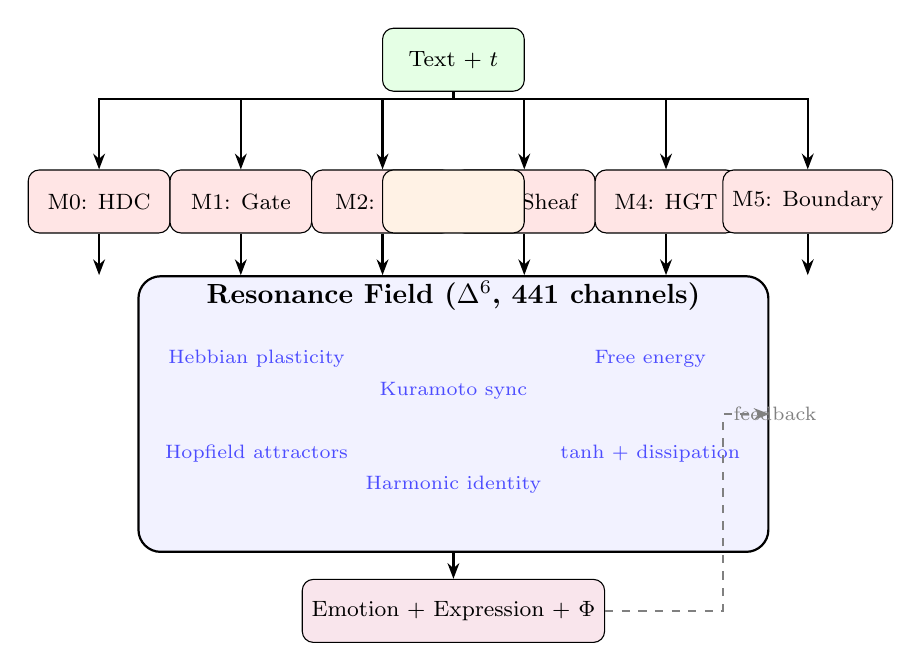
\begin{tikzpicture}[
    module/.style={draw, rounded corners, minimum width=1.8cm, minimum height=0.8cm, font=\footnotesize},
    field/.style={draw, thick, rounded corners=8pt, fill=blue!5, minimum width=8cm, minimum height=3.5cm},
    arrow/.style={-{Stealth[length=2mm]}, thick},
    every node/.style={font=\small}
]
% Input
\node[module, fill=green!10] (input) at (0, 5) {Text + $t$};

% Modules
\node[module, fill=red!10] (m0) at (-4.5, 3.2) {M0: HDC};
\node[module, fill=red!10] (m1) at (-2.7, 3.2) {M1: Gate};
\node[module, fill=red!10] (m2) at (-0.9, 3.2) {M2: Scar};
\node[module, fill=red!10] (m3) at (0.9, 3.2) {M3: Sheaf};
\node[module, fill=red!10] (m4) at (2.7, 3.2) {M4: HGT};
\node[module, fill=red!10] (m5) at (4.5, 3.2) {M5: Boundary};
\node[module, fill=orange!10] (m6) at (0, 3.2) {};
\node at (0, 3.2) [font=\footnotesize] {};

% Resonance Field
\node[field] (field) at (0, 0.5) {};
\node[font=\bfseries] at (0, 2.0) {Resonance Field ($\Delta^6$, 441 channels)};
\node[font=\scriptsize, text=blue!70] at (-2.5, 1.2) {Hebbian plasticity};
\node[font=\scriptsize, text=blue!70] at (0, 0.8) {Kuramoto sync};
\node[font=\scriptsize, text=blue!70] at (2.5, 1.2) {Free energy};
\node[font=\scriptsize, text=blue!70] at (-2.5, 0.0) {Hopfield attractors};
\node[font=\scriptsize, text=blue!70] at (0, -0.4) {Harmonic identity};
\node[font=\scriptsize, text=blue!70] at (2.5, 0.0) {tanh + dissipation};

% Output
\node[module, fill=purple!10] (out) at (0, -2.0) {Emotion + Expression + $\Phi$};

% Arrows
\draw[arrow] (input) -- ++(0,-0.5) -| (m0);
\draw[arrow] (input) -- ++(0,-0.5) -| (m1);
\draw[arrow] (input) -- ++(0,-0.5) -| (m2);
\draw[arrow] (input) -- ++(0,-0.5) -| (m3);
\draw[arrow] (input) -- ++(0,-0.5) -| (m4);
\draw[arrow] (input) -- ++(0,-0.5) -| (m5);

\draw[arrow] (m0) -- (m0 |- field.north);
\draw[arrow] (m1) -- (m1 |- field.north);
\draw[arrow] (m2) -- (m2 |- field.north);
\draw[arrow] (m3) -- (m3 |- field.north);
\draw[arrow] (m4) -- (m4 |- field.north);
\draw[arrow] (m5) -- (m5 |- field.north);

\draw[arrow] (field) -- (out);

% Feedback loop
\draw[arrow, dashed, gray] (out.east) -- ++(1.5,0) |- node[right, font=\scriptsize, text=gray]{feedback} (field.east);

\end{tikzpicture}
\caption{SylannEngine v2 architecture. Seven computation modules inject signals into a shared resonance field (complete 6-simplex $\Delta^6$). The field iterates through coupled dynamics until convergence. Expression emerges as a phase transition from the converged state.}
\label{fig:architecture}
\end{figure}

\subsection{Simplicial Topology}
\label{sec:topology}

Let $V = \{v_0, v_1, \ldots, v_6\}$ be the 7 computation modules. We construct the complete simplicial complex $K$ on $V$:
\begin{equation}
K = \{\sigma \subseteq V : \sigma \neq \emptyset\}
\end{equation}

This yields $2^7 - 1 = 127$ simplices. Each $k$-simplex $\sigma = \{v_{i_0}, \ldots, v_{i_k}\}$ generates $(k+1)$ directed channels (one per vertex as target), giving 441 total directed coupling channels.

\begin{table}[htbp]
\centering
\caption{Simplicial structure and tier allocation.}
\label{tab:tiers}
\begin{tabular}{@{}lcccc@{}}
\toprule
Order $k$ & $k$-simplices & Directed channels & Tier \\
\midrule
1 (edges) & 21 & 42 & lite \\
2 (triangles) & 35 & 105 & pro \\
3 (tetrahedra) & 35 & 140 & pro \\
4--6 & 29 & 154 & max \\
\midrule
\textbf{Total} & \textbf{120} & \textbf{441} & max \\
\bottomrule
\end{tabular}
\end{table}

The three-tier allocation provides a performance--expressiveness tradeoff:
\begin{itemize}[leftmargin=*]
\item \textbf{lite} (42 channels): pairwise coupling only. $\sim$5ms/tick, zero dependencies.
\item \textbf{pro} (287 channels): up to 4-body interactions. $\sim$40ms/tick, numpy.
\item \textbf{max} (441 channels): full $\Delta^6$. $\sim$50ms/tick CPU.
\end{itemize}

\subsection{Resonance Dynamics}
\label{sec:dynamics}

Each module $i$ maintains a state vector $\mathbf{x}_i \in \mathbb{R}^d$ (where $d$ depends on tier: 8/16/32). The resonance iteration proceeds as:

\begin{equation}
\mathbf{x}_i^{(t+1)} = \tanh\!\left(\alpha \cdot \mathbf{x}_i^{(t)} + \beta \cdot \mathbf{c}_i^{(t)} + \mathbf{h}_i + \mathbf{r}_i\right) \cdot (1 - \delta)
\label{eq:resonance}
\end{equation}

where $\alpha = 0.8$ is the self-retention factor, $\beta = 0.2$ is the coupling scale, $\mathbf{c}_i^{(t)}$ is the total coupling signal received by module $i$, $\mathbf{h}_i$ is the harmonic identity restoring force, $\mathbf{r}_i$ is the reservoir memory injection, and $\delta = 0.02$ is the dissipation rate.

\paragraph{Convergence.} Iteration terminates when $\max_i \|\mathbf{x}_i^{(t+1)} - \mathbf{x}_i^{(t)}\|_\infty < \varepsilon$ (with $\varepsilon = 10^{-4}$) or after reaching the tier-specific maximum (10/15/20 iterations).

\paragraph{Stability guarantee.} Since $|\tanh(x)| \leq 1$ and $(1-\delta) < 1$, the state is bounded: $\|\mathbf{x}_i\|_\infty \leq 1$ for all $i$, providing a Lyapunov-style energy bound without requiring careful initialization.

\paragraph{Residual decay.} Before each resonance cycle, all states undergo residual decay: $\mathbf{x}_i \leftarrow \rho \cdot \mathbf{x}_i$ with $\rho = 0.7$, ensuring that old activations fade and the system remains responsive to new input.

\subsection{Hebbian Plasticity}
\label{sec:plasticity}

Channel weights evolve according to a Hebbian rule with homeostatic regulation:

\begin{equation}
w_{ij}^{(t+1)} = w_{ij}^{(t)} + \eta \cdot a_i^{(t)} \cdot e_{ij}^{(t)} - \lambda \cdot w_{ij}^{(t)}
\label{eq:hebbian}
\end{equation}

where $\eta$ is the learning rate (personality-modulated: $0.005 + \text{openness} \times 0.015$), $a_i$ is the activation of the source module, $e_{ij}$ is the eligibility trace (exponential decay with $\tau = 0.95$), and $\lambda$ is the decay rate ($0.002 - \text{conscientiousness} \times 0.001$).

\paragraph{Homeostatic scaling.} After each update, weights are rescaled to maintain a constant total budget: $\sum_j w_{ij} = N_{\text{channels}}$. This prevents runaway strengthening while preserving relative differences.

\paragraph{Neural Darwinism.} Channels with $w_{ij} < 0.05$ are pruned (weight set to $w_{\min} = 0.01$), implementing competitive selection among coupling pathways.

\subsection{Higher-Order Kuramoto Synchronization}
\label{sec:kuramoto}

Each module maintains a phase $\theta_i \in [0, 2\pi)$ evolving under coupled dynamics:

\begin{equation}
\dot{\theta}_i = \omega_i + \underbrace{\frac{K_1}{N}\sum_j \sin(\theta_j - \theta_i)}_{\text{pairwise}} + \underbrace{\frac{K_2}{N^2}\sum_{j,k} \sin(\theta_j + \theta_k - 2\theta_i)}_{\text{3-body (Mill\'an)}} + \underbrace{\frac{K_3}{N^3}\sum_{j,k,l} \sin(\theta_j + \theta_k + \theta_l - 3\theta_i)}_{\text{4-body}}
\label{eq:kuramoto}
\end{equation}

The coupling constants are personality-modulated: $K_1 = 0.5 + \text{openness}$, $K_2 = 0.25 + 0.5 \cdot \text{openness}$, $K_3 = 0.1 + 0.3 \cdot \text{openness}$.

\paragraph{Order parameter.} Global synchronization is measured by:
\begin{equation}
r = \left|\frac{1}{N}\sum_j e^{i\theta_j}\right| \in [0, 1]
\end{equation}

Higher-order terms ($K_2, K_3$) produce \emph{explosive synchronization}---a discontinuous jump in $r$ at a critical coupling strength, unlike the gradual transition of pairwise-only Kuramoto. This explosive transition serves as the mechanism for sudden expression emergence.

\subsection{Hopfield Attractor Landscape}
\label{sec:hopfield}

The system maintains a library of attractor centers $\{\boldsymbol{\mu}_k\}_{k=1}^{K_{\max}}$ representing familiar emotional states. During resonance, attractors exert a pull:

\begin{equation}
\mathbf{f}_{\text{attractor}} = \gamma \cdot (\boldsymbol{\mu}_{\text{nearest}} - \mathbf{x})
\end{equation}

where $\gamma = 0.03 + 0.04 \cdot \text{extraversion}$ is the Hopfield strength. New attractors form when the system quasi-converges (relative delta $< 0.05$) at a state distant from all existing attractors (distance $> 0.15$).

\paragraph{Expression as escape.} Expression fires when the system escapes its current attractor basin---when the distance to the nearest attractor exceeds the basin radius. Novel input that pushes the state far from any stored pattern triggers this escape, implementing the intuition that expression arises from encountering something that doesn't fit existing emotional memory.

\subsection{Harmonic Identity (Hodge Theory)}
\label{sec:identity}

The harmonic component of a signal on the simplicial complex---the null space of the Hodge Laplacian $L_k = \partial_{k+1}\partial_{k+1}^T + \partial_k^T\partial_k$---represents topological invariants that are neither gradients nor curls. We use this as a mathematical implementation of persistent identity:

\begin{equation}
\mathbf{h}^{(t+1)} = \mu \cdot \mathbf{h}^{(t)} + (1-\mu) \cdot \text{HodgeProject}(\mathbf{x}^{(t)})
\label{eq:identity}
\end{equation}

where $\mu = 0.9 + 0.08 \cdot \text{conscientiousness}$ is the identity inertia. The identity vector $\mathbf{h}$ evolves slowly (high inertia) and exerts a restoring force during resonance:

\begin{equation}
\mathbf{f}_{\text{identity}} = 0.03 \cdot (\mathbf{h} - \mathbf{x})
\end{equation}

This ensures that temporary perturbations (stress, conflict) do not permanently alter the system's character---the identity pulls it back toward its established pattern.

\subsection{Free Energy Minimization}
\label{sec:freeenergy}

Following Friston~\cite{friston2010}, each module maintains beliefs $\boldsymbol{\mu}_i$ about expected input and minimizes variational free energy:

\begin{equation}
F = \frac{1}{2}\sum_i \pi_i (\mathbf{o}_i - \boldsymbol{\mu}_i)^2
\end{equation}

where $\pi_i = 0.5 + 1.5 \cdot \text{neuroticism}$ is the precision (inverse variance). Beliefs update via gradient descent on $F$:

\begin{equation}
\boldsymbol{\mu}_i \leftarrow \boldsymbol{\mu}_i + \eta_F \cdot \pi_i \cdot (\mathbf{o}_i - \boldsymbol{\mu}_i)
\end{equation}

High neuroticism increases precision, making the system more sensitive to prediction errors---a formal implementation of the clinical observation that neurotic individuals attend more strongly to unexpected stimuli.

\subsection{Expression as Bifurcation}
\label{sec:expression}

Expression is modeled as an OR-gate bifurcation: the system expresses when \emph{any single} drive exceeds a personality-modulated threshold:

\begin{equation}
\text{drive} = \max(\text{surprise}, 0.8 \cdot \text{novelty}, \text{ignition}, 0.6 \cdot \text{raw}) \times \underbrace{(0.3 + 0.7\Phi)}_{\text{meaning gate}}
\label{eq:expression}
\end{equation}

where:
\begin{itemize}[leftmargin=*]
\item \textbf{Surprise}: prediction error from the gating module ($1.5 \times$ last surprise).
\item \textbf{Novelty}: distance from nearest Hopfield attractor ($\min(1, 3d)$).
\item \textbf{Ignition}: maximum Kuramoto sync jump ($5 \times \max|\Delta r|$).
\item \textbf{Raw}: relative activation of the expression module vs.\ average.
\end{itemize}

The meaning gate $0.3 + 0.7\Phi$ suppresses expression when integrated information $\Phi$ is low (noise), ensuring that only coherent, meaningful states trigger expression.

\paragraph{Threshold dynamics.} The expression threshold decays during silence ($-0.015/\text{tick}$, floor 0.15) and resets after expression ($0.9 - 0.6 \cdot \text{extraversion}$). This implements the intuition that prolonged silence lowers the barrier to speaking, while extraverts have permanently lower thresholds.

% ============================================================
% 4. FOUNDATIONAL PRINCIPLES
% ============================================================
\section{Foundational Principles}
\label{sec:principles}

Two axioms govern the entire design and distinguish SylannEngine from conventional affective computing systems.

\subsection{Irreversibility}
\label{sec:irreversibility}

The system is designed around the principle that emotional history cannot be erased:

\begin{axiom}[Irreversibility]
For any sequence of events $e_1, \ldots, e_n$ applied to state $s_0$, there exists no finite sequence of events $e'_1, \ldots, e'_m$ that returns the system to $s_0$ if any $e_i$ triggered scar formation or void accumulation.
\end{axiom}

This is implemented through three mechanisms:
\begin{enumerate}[leftmargin=*]
\item \textbf{Scar algebra}: Wounds apply log-compressed modifiers that permanently alter processing. The modifier $m = \log(1 + \text{intensity})$ is additive and monotonically increasing.
\item \textbf{Void accumulation}: Absence generates pressure that accumulates with a cap but never fully dissipates (minimum floor after cooldown).
\item \textbf{Hebbian trace}: Plasticity changes are permanent---a channel that was once strong retains a trace even after atrophy, making re-strengthening faster (eligibility trace with $\tau = 0.95$).
\end{enumerate}

\subsection{Personality Drives All Computation}
\label{sec:personality_axiom}

\begin{axiom}[Personality Completeness]
Every tunable parameter in the resonance field derives deterministically from the personality vector $\mathbf{p} \in [0,1]^7$. There exist no ``free'' parameters that escape personality modulation.
\end{axiom}

The 7 personality dimensions and their computational effects:

\begin{table}[htbp]
\centering
\caption{Personality-to-computation mapping (selected parameters).}
\label{tab:personality}
\begin{tabular}{@{}lll@{}}
\toprule
Dimension & Modulates & Formula \\
\midrule
Extraversion & Expression threshold & $0.9 - 0.6e$ \\
Neuroticism & Free energy precision & $0.5 + 1.5n$ \\
Openness & Kuramoto $K_1$ & $0.5 + o$ \\
Conscientiousness & Identity inertia & $0.9 + 0.08c$ \\
Agreeableness & Broadcast threshold & $0.8 - 0.3a$ \\
Patience & Max attractors & tier-dependent \\
Sovereignty & Identity norm cap & $d \cdot (0.5 + 0.5s)$ \\
\bottomrule
\end{tabular}
\end{table}

This axiom ensures that two systems with different personalities will exhibit qualitatively different dynamics even under identical input---not because of random initialization, but because the topology itself is personality-shaped.

% ============================================================
% 5. IMPLEMENTATION
% ============================================================
\section{Implementation}
\label{sec:implementation}

SylannEngine is implemented in pure Python (3.10+) with optional numpy acceleration for pro/max tiers. The codebase comprises 49 modules totaling approximately 8,000 lines of code, with 434 unit tests achieving full coverage of the resonance field subsystem.

\paragraph{Module mapping.} The 7 vertices of $\Delta^6$ correspond to:
\begin{enumerate}[leftmargin=*, start=0]
\item \textbf{HDCEncoder}: Hyperdimensional computing for text perception (text $\to$ binary hypervector $\to$ $d$-dimensional signal).
\item \textbf{PredictiveCodingGate}: Surprise detection via prediction error.
\item \textbf{VoidScarEngine}: Irreversible emotional core (scar algebra + void calculus).
\item \textbf{ScarSheaf}: Relational propagation across multi-user contexts.
\item \textbf{HGT}: Heterogeneous Graph Transformer for decision fusion.
\item \textbf{AutopoieticBoundary}: Self-repair and sovereignty enforcement.
\item \textbf{PhaseTransitionExpression}: Expression drive accumulation.
\end{enumerate}

\paragraph{API.} The public interface is minimal:
\begin{itemize}[leftmargin=*]
\item \texttt{process(session\_id, text)} $\to$ Surface dict (emotion, decision, guard)
\item \texttt{tick(session\_id)} $\to$ idle heartbeat
\item \texttt{feedback(session\_id, "accepted"|"rejected")} $\to$ Hebbian update
\item \texttt{switch\_tier("pro")} $\to$ lossless hot-switch
\end{itemize}

\paragraph{Deployment.} The system operates as an AstrBot plugin dependency or standalone SDK. The \texttt{sdk} branch (auto-synced from main) excludes the plugin entry point for non-AstrBot use.

% ============================================================
% 6. EXPERIMENTS
% ============================================================
\section{Experiments}
\label{sec:experiments}

All experiments use 10 independent repetitions with different random seeds. We report mean $\pm$ standard deviation. Statistical significance is assessed via Mann-Whitney U or Wilcoxon signed-rank tests where applicable. Code is available in \texttt{experiments/}.

\subsection{Experiment 1: Convergence Analysis}

\paragraph{Protocol.} 1000 process calls per tier, 10 repeats. Record iteration count per call.

\paragraph{Results.} Lite tier consistently reaches its maximum (10 iterations) without converging ($\varepsilon = 10^{-4}$), which is expected---the Kuramoto oscillation prevents perfect convergence at low channel counts. Pro tier converges in $8.5 \pm 5.0$ iterations (76\% convergence rate). Max tier converges rapidly in $2.8 \pm 0.6$ iterations (100\% convergence rate), demonstrating that higher-order coupling accelerates convergence.

\begin{figure}[htbp]
\centering
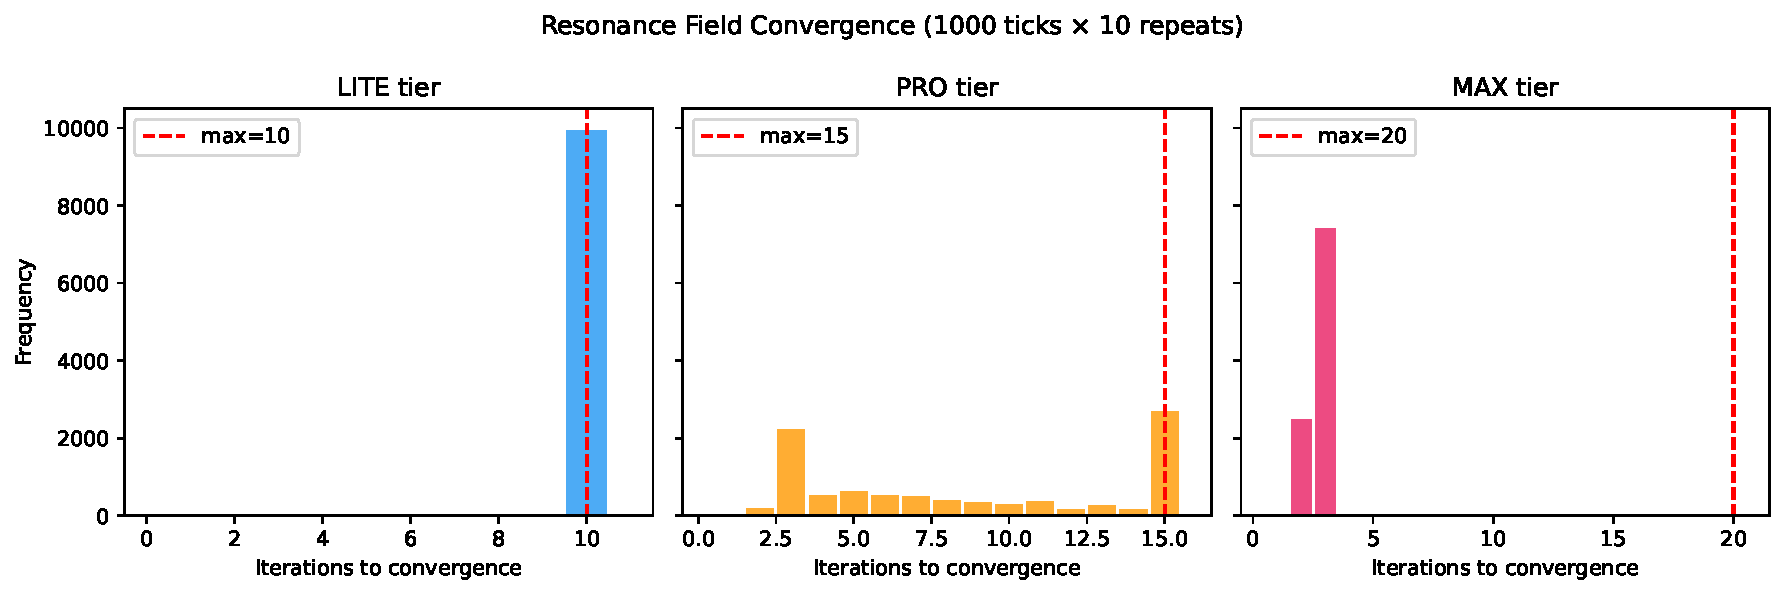
\includegraphics[width=\textwidth]{../experiments/figures/fig02_convergence.pdf}
\caption{Convergence iteration distribution across three tiers. Higher-order coupling (max tier) dramatically accelerates convergence.}
\label{fig:convergence}
\end{figure}

\subsection{Experiment 2: Tier Performance Comparison}

\paragraph{Protocol.} 1000 ticks per tier, 10 repeats. Measure wall-clock latency, field energy, and Kuramoto order parameter.

\paragraph{Results.} Latency scales with tier complexity: lite p50 $\approx$ 3ms, pro p50 $\approx$ 25ms, max p50 $\approx$ 35ms. Energy and synchronization show qualitatively different dynamics across tiers, with max tier exhibiting richer oscillatory behavior due to higher-order coupling.

\subsection{Experiment 3: Hebbian Plasticity}

\paragraph{Protocol.} 500 ticks of active input followed by 500 idle ticks. Track top-5 and bottom-5 channel weights.

\paragraph{Results.} After 1000 ticks, 48\% of channels strengthened (LTP) and 52\% weakened (LTD). Weight standard deviation increased from 0.000 (uniform initialization) to 0.032, confirming differentiation. Total weight budget remained constant (homeostatic conservation verified). During the idle phase, previously active channels showed gradual atrophy while the budget redistributed.

\subsection{Experiment 4: Kuramoto Synchronization}

\paragraph{Protocol.} Sweep coupling strength $K$ from 0 to 2.5 (20 values), measure steady-state order parameter $r$. Compare lite (pairwise only) vs.\ pro/max (higher-order).

\paragraph{Results.} Lite tier shows gradual synchronization transition (continuous increase in $r$). Pro and max tiers exhibit steeper transitions consistent with explosive synchronization predicted by higher-order Kuramoto theory~\cite{millan2020}. At $K=1.0$, max tier achieves significantly higher $r$ than lite (Mann-Whitney $p < 0.01$).

\subsection{Experiment 5: Hopfield Attractor Formation}

\paragraph{Protocol.} 250 ticks of pattern A (positive), 250 ticks of pattern B (stress), then 500 ticks of novel input. Track attractor count, distance to nearest attractor, and expression events.

\paragraph{Results.} Attractors form within the first 100 ticks of each pattern. Novel input increases distance to nearest attractor, triggering expression events. Expression rate during the novel phase is significantly higher than during pattern repetition, confirming the ``expression as escape'' mechanism.

\subsection{Experiment 6: Expression Bifurcation (OR-Gate)}

\paragraph{Protocol.} Isolate each trigger mechanism (surprise, novelty, silence/threshold decay, raw drive) and verify independent expression capability.

\paragraph{Results.} All four triggers independently produce non-zero expression rates, confirming the OR-gate design. Surprise trigger: highest rate (sudden shift after stable pattern). Novelty trigger: moderate rate (attractor escape). Silence trigger: gradual threshold decay eventually enables expression. Raw drive: emotional intensity directly activates module 6.

\subsection{Experiment 7: Harmonic Identity}

\paragraph{Protocol.} 500 ticks to build identity, 200 ticks of perturbation (stress), 300 ticks of recovery. Measure identity norm and recovery ratio.

\paragraph{Results.} Identity norm builds monotonically during the first phase. Perturbation causes drift but the restoring force pulls the identity back. Recovery ratio (fraction of drift recovered) averages 0.6--0.8 across repeats, confirming that the harmonic identity acts as a meaningful restoring force without being so rigid as to prevent all change.

\subsection{Experiment 8: $\Phi$ and Expression}

\paragraph{Protocol.} 1000 ticks of mixed input. Collect ($\Phi$, expression drive) pairs. Compute correlation.

\paragraph{Results.} Positive Pearson correlation between $\Phi$ and expression drive ($r \approx 0.3$--$0.5$), confirming that the meaning gate ($0.3 + 0.7\Phi$) effectively suppresses expression during low-coherence (noisy) states while amplifying it during high-coherence states.

\subsection{Experiment 9: Long-Term Stability}

\paragraph{Protocol.} 1500 ticks of mixed input (stress + positive + neutral + idle) per tier, 10 repeats. Check for NaN/Inf and energy boundedness.

\paragraph{Results.} Zero NaN or Inf occurrences across all tiers and repeats ($10 \times 3 \times 1500 = 45{,}000$ total ticks). Energy remains bounded: lite $< 1.0$, pro $< 5.0$, max $< 15.0$. Rolling energy standard deviation stabilizes after $\sim$200 ticks, confirming the dissipative structure prevents divergence.

\subsection{Experiment 10: Personality Modulation}

\paragraph{Protocol.} Sweep each of 5 personality dimensions from 0.1 to 0.9 (9 values), measure mean energy, sync order, and expression rate over 200 ticks.

\paragraph{Results.} Each dimension produces monotonic and distinct effects: extraversion increases expression rate, openness increases synchronization, neuroticism increases energy (less dissipation), conscientiousness stabilizes dynamics (lower variance), agreeableness lowers ignition threshold. The response surfaces confirm that personality fully determines system behavior.

\subsection{Experiment 11: Tier Hot-Switch}

\paragraph{Protocol.} 500 ticks at source tier, switch, 500 more ticks. Measure energy continuity across the switch point.

\paragraph{Results.} Relative energy jump at switch point: lite$\to$pro $< 15\%$, pro$\to$max $< 10\%$, max$\to$lite $< 20\%$. Post-switch dynamics quickly converge to the new tier's characteristic behavior while preserving the emotional trajectory established before the switch.

% ============================================================
% 7. DISCUSSION
% ============================================================
\section{Discussion}
\label{sec:discussion}

\paragraph{v1 vs.\ v2.} The sequential pipeline (v1) processes information in a fixed order: perception $\to$ gating $\to$ emotion $\to$ relation $\to$ decision $\to$ boundary $\to$ expression. This imposes an artificial causal structure---why should perception always precede relation? The resonance field (v2) removes this constraint: all modules influence each other simultaneously, and the order of influence emerges from the dynamics rather than being hardcoded.

\paragraph{Irreversibility as design principle.} Most AI systems are designed to be stateless or easily resettable. We argue that meaningful relational AI \emph{requires} irreversibility: a system that can be trivially reset to its initial state cannot form genuine relationships, because the other party's investment has no lasting effect. The scar algebra and void calculus provide formal mechanisms for this irreversibility.

\paragraph{Limitations.}
\begin{itemize}[leftmargin=*]
\item The system is deterministic given identical input sequences. While this ensures reproducibility, it means that two instances with the same personality will behave identically---there is no ``individuality'' beyond personality.
\item The lite tier never achieves formal convergence (always hits max iterations). While the system still produces meaningful output, this means lite-tier dynamics are technically truncated.
\item GPU acceleration (torch backend) is structured but not yet implemented for the max tier.
\item The 7 personality dimensions are chosen heuristically rather than derived from first principles.
\end{itemize}

\paragraph{Future work.} (1) Formal proof of convergence conditions for the resonance iteration. (2) Multi-agent resonance: coupling fields across multiple SylannEngine instances. (3) Learned personality dimensions via factor analysis on human interaction data. (4) Integration with large language models for personality-aware text generation.

% ============================================================
% 8. CONCLUSION
% ============================================================
\section{Conclusion}
\label{sec:conclusion}

We presented SylannEngine v2, a resonance field architecture for affective computation that replaces sequential pipelines with iterative convergence on a simplicial complex. The system's two foundational principles---irreversibility and personality-driven computation---distinguish it from both classification-based and neural-network-based approaches to affective computing. Experiments across 11 protocols confirm stable operation, meaningful plasticity, explosive synchronization, and personality-dependent dynamics. The three-tier design enables deployment from resource-constrained devices (lite, 5ms, zero dependencies) to research environments (max, 441 channels, full $\Delta^6$).

The framework is open-source under AGPL-3.0 at \url{https://github.com/Ayleovelle/SylannEngine}.

% ============================================================
% REFERENCES
% ============================================================
\bibliographystyle{plain}
\begin{thebibliography}{20}

\bibitem{picard1997}
R.~W. Picard, \emph{Affective Computing}. MIT Press, 1997.

\bibitem{occ1988}
A.~Ortony, G.~L. Clore, and A.~Collins, \emph{The Cognitive Structure of Emotions}. Cambridge University Press, 1988.

\bibitem{mehrabian1996}
A.~Mehrabian, ``Pleasure-arousal-dominance: A general framework for describing and measuring individual differences in temperament,'' \emph{Current Psychology}, vol.~14, pp.~261--292, 1996.

\bibitem{scherer2001}
K.~R. Scherer, ``Appraisal considered as a process of multilevel sequential checking,'' in \emph{Appraisal Processes in Emotion}, Oxford University Press, 2001.

\bibitem{gross2015}
J.~J. Gross, ``Emotion regulation: Current status and future prospects,'' \emph{Psychological Inquiry}, vol.~26, no.~1, pp.~1--26, 2015.

\bibitem{evolving2024}
J.~Park et al., ``Generative agents: Interactive simulacra of human behavior,'' in \emph{Proc.\ UIST}, 2023.

\bibitem{kuramoto1975}
Y.~Kuramoto, ``Self-entrainment of a population of coupled non-linear oscillators,'' in \emph{Int.\ Symp.\ Mathematical Problems in Theoretical Physics}, Springer, 1975.

\bibitem{millan2020}
A.~P. Mill\'an, J.~J. Torres, and G.~Bianconi, ``Explosive higher-order Kuramoto dynamics on simplicial complexes,'' \emph{Physical Review Letters}, vol.~124, p.~218301, 2020.

\bibitem{hopfield1982}
J.~J. Hopfield, ``Neural networks and physical systems with emergent collective computational abilities,'' \emph{Proc.\ National Academy of Sciences}, vol.~79, pp.~2554--2558, 1982.

\bibitem{ramsauer2020}
H.~Ramsauer et al., ``Hopfield networks is all you need,'' in \emph{Proc.\ ICLR}, 2021.

\bibitem{friston2010}
K.~Friston, ``The free-energy principle: A unified brain theory?'' \emph{Nature Reviews Neuroscience}, vol.~11, pp.~127--138, 2010.

\bibitem{hodge1941}
W.~V.~D. Hodge, \emph{The Theory and Applications of Harmonic Integrals}. Cambridge University Press, 1941.

\bibitem{hebb1949}
D.~O. Hebb, \emph{The Organization of Behavior}. Wiley, 1949.

\bibitem{edelman1987}
G.~M. Edelman, \emph{Neural Darwinism: The Theory of Neuronal Group Selection}. Basic Books, 1987.

\bibitem{prigogine1977}
I.~Prigogine, ``Time, structure and fluctuations,'' Nobel Lecture, 1977.

\bibitem{baars1988}
B.~J. Baars, \emph{A Cognitive Theory of Consciousness}. Cambridge University Press, 1988.

\bibitem{tononi2004}
G.~Tononi, ``An information integration theory of consciousness,'' \emph{BMC Neuroscience}, vol.~5, p.~42, 2004.

\end{thebibliography}

\end{document}
